%% =====================================================================
%% DeepCARE -- MDPI *Life* (ISSN 2075-1729)
%% Supplementary Materials
%% Built on the SAME MDPI article template as main.tex: mdpi.cls with the
%% official "supfile" document type.  supfile automatically typesets
%%   "Supplementary Materials: <Title>" + the full \Author line,
%%   renumbers figures/tables as S1, S2, ... and prints the S-page header.
%% v9.8 / 2026-11-10 : MDPI template, full 16-author roster, affiliations,
%%   equal-contribution and corresponding footnotes, CRediT, funding,
%%   data availability, AI statement and conflicts of interest.
%% v9.9 / 2026-11-10 : layout fix.  The supfile branch of mdpi.cls prints only
%%   \maketitle (title + authors) and skips \maketitlen, which is the command
%%   that actually typesets \address / \corres / \firstnote.  Call \maketitlen
%%   explicitly so the affiliation block appears in the cover area, and add
%%   \vspace{14pt} to offset the hard-coded \vspace{-8pt} at the start of
%%   \abstractkeywords (that -8pt normally cancels \maketitlen's trailing
%%   space; without \maketitlen it pulled the Abstract flush against the
%%   author line).
%% Compile: pdflatex supplement.tex  (twice, for LastPage/refs)
%% Dependencies (shared with main.tex): mdpi.cls, Definitions/, figures/
%% =====================================================================

\documentclass[life,supfile,submit,pdftex,moreauthors]{mdpi}

\usepackage{graphicx}
\graphicspath{{figures/}}
\usepackage{amsmath,amssymb}
\usepackage{booktabs}
\usepackage{multirow}
\usepackage{array}
\usepackage{float}
\usepackage{lastpage}
\setlength{\headheight}{20pt}
\emergencystretch=1em
\renewcommand{\topfraction}{0.9}
\renewcommand{\textfraction}{0.05}
\renewcommand{\floatpagefraction}{0.8}

%% ---- Volume / page placeholders (final values are assigned by the EO) ----
\firstpage{1}
\pubvolume{1}
\issuenum{1}
\articlenumber{0}
\pubyear{2026}
\copyrightyear{2026}
\datereceived{ }
\daterevised{ }
\dateaccepted{ }
\datepublished{ }
\doinum{}

%% ---- Title and the full author list (mdpi.cls prints both on the cover) ----
\Title{DeepCARE: Transferable assessment of clinically relevant allergen cross-reactivity for unseen pairs using a protein foundation language model-based deep learning framework}
\TitleCitation{DeepCARE: Transferable assessment of clinically relevant allergen cross-reactivity for unseen pairs using a protein foundation language model-based deep learning framework}

\Author{Tongfei Shen $^{1,2,\dagger}$, Jie Liu $^{1,\dagger}$, Ziao Pan $^{1,\dagger}$, Peng Li $^{1,\dagger}$, Xiujuan Leng $^{1}$, Ge Wang $^{1}$, Jichao Zhang $^{1}$, Fuquan Yi $^{1}$, Zheng Xiang $^{1}$, Yuxiang Liu $^{1}$, Wenjing Song $^{1}$, Shuyan Ma $^{1}$, Yuyue Cui $^{1}$, Haoran Wang $^{1}$, Yurong Qin $^{3,*}$, Shouqiang Sun $^{1,*}$}
\AuthorNames{Tongfei Shen; Jie Liu; Ziao Pan; Peng Li; Xiujuan Leng; Ge Wang; Jichao Zhang; Fuquan Yi; Zheng Xiang; Yuxiang Liu; Wenjing Song; Shuyan Ma; Yuyue Cui; Haoran Wang; Yurong Qin; Shouqiang Sun}
\AuthorCitation{Shen, T.; Liu, J.; Pan, Z.; Li, P.; Leng, X.; Wang, G.; Zhang, J.; Yi, F.; Xiang, Z.; Liu, Y.; Song, W.; Ma, S.; Cui, Y.; Wang, H.; Qin, Y.; Sun, S}

\address{%
$^{1}$\quad School of Information Science and Engineering, Qingdao Huanghai University, Qingdao 266427, Shandong, China\\
$^{2}$\quad Department of Computer Science, City University of Hong Kong, Kowloon, Hong Kong SAR, China\\
$^{3}$\quad School of Food and Drugs, Shenzhen Polytechnic University, Shenzhen 518055, China\\
}

\corres{Correspondence: qinyurong@szpu.edu.cn (Yurong Qin); sunsq@qdhhc.edu.cn (Shouqiang Sun).}

\firstnote{These authors contributed equally to this work.}

\abstract{This supplement carries the extended comparisons and the full protocol
record referenced by the main manuscript: the per-seed metric record that the
main body averages, the identity-oracle contrast array, the carried calibration
cells, the recorded screens with their verdicts, and the construction, split,
and provenance record of the data pipeline. It accompanies the article
``DeepCARE: Transferable assessment of clinically relevant allergen
cross-reactivity for unseen pairs using a protein foundation language
model-based deep learning framework'' submitted to \textit{Life}. On the
family-stratified holdout of 73 never-trained clinical pairs, the ensemble
attained an AUPRC of 0.647 against 0.242 for the homology baseline and an
AUROC of 0.799 against 0.552. Figures S1--S2 reproduce these comparisons in
their per-seed form and document the protocol fixed before holdout contact.
All reported values reproduce from the frozen scoring tables and the analysis
code released with the manuscript.}

\keyword{Allergen cross-reactivity; Protein language models; Deep learning; Imbalanced biomedical data; Ranking calibration; Interpretable screening}

\begin{document}
\nolinenumbers  % "submit" status turns line numbers on; supplementary is cleaner without them

%% mdpi.cls runs \maketitle (title + authors) automatically for supfile, but
%% SKIPS \maketitlen -- the command that typesets \address, \corres and
%% \firstnote.  Restore the standard article order explicitly.
\maketitlen
\let\maketitlen\relax
%% \abstractkeywords starts with a hard-coded \vspace{-8pt} that normally
%% cancels \maketitlen's trailing space.  Net +6pt here keeps a clear gap
%% between the affiliation/footnote block and the Abstract.
\vspace{14pt}
\abstractkeywords

\vspace{10pt}
{\fontsize{9}{11.5}\selectfont
\noindent\textbf{Manuscript.} This is the Supplementary Material accompanying
the article \textit{DeepCARE: Transferable assessment of clinically relevant
allergen cross-reactivity for unseen pairs using a protein foundation language
model-based deep learning framework}, submitted to \textit{Life} (MDPI). It
contains Figures S1--S2 and Sections S1--S3. The LaTeX source, the two
supplementary figures, a released data slice, the frozen scoring tables and
the analysis code are openly available at
\url{https://github.com/SHENTongfei/DeepCARE}.

\vspace{6pt}
\noindent\textbf{Author abbreviations (16 authors, in manuscript order).}
Tongfei Shen $^{1,2,\dagger}$ (T.S.);
Jie Liu $^{1,\dagger}$ (J.L.);
Ziao Pan $^{1,\dagger}$ (Z.P.);
Peng Li $^{1,\dagger}$ (P.L.);
Xiujuan Leng $^{1}$ (X.L.);
Ge Wang $^{1}$ (G.W.);
Jichao Zhang $^{1}$ (J.Z.);
Fuquan Yi $^{1}$ (F.Y.);
Zheng Xiang $^{1}$ (Z.X.);
Yuxiang Liu $^{1}$ (Y.L.);
Wenjing Song $^{1}$ (W.S.);
Shuyan Ma $^{1}$ (S.M.);
Yuyue Cui $^{1}$ (Y.C.);
Haoran Wang $^{1}$ (H.W.);
Yurong Qin $^{3,*}$ (Y.Q.);
Shouqiang Sun $^{1,*}$ (S.S.).

\vspace{6pt}
\noindent\textbf{$^{\dagger}$ Joint first authors.}
Tongfei Shen, Jie Liu, Ziao Pan and Peng Li contributed equally to this work.
The three numbered affiliations and the $^{*}$ corresponding-author
addresses are given in the cover block above, following the same layout as
the main manuscript; the full CRediT statement appears at the end of this file.
}

\vspace{12pt}

%% =====================================================================
\section*{S1. Extended comparisons and the full per-metric record}
\label{secS1}

\begin{figure}[H]
\centering
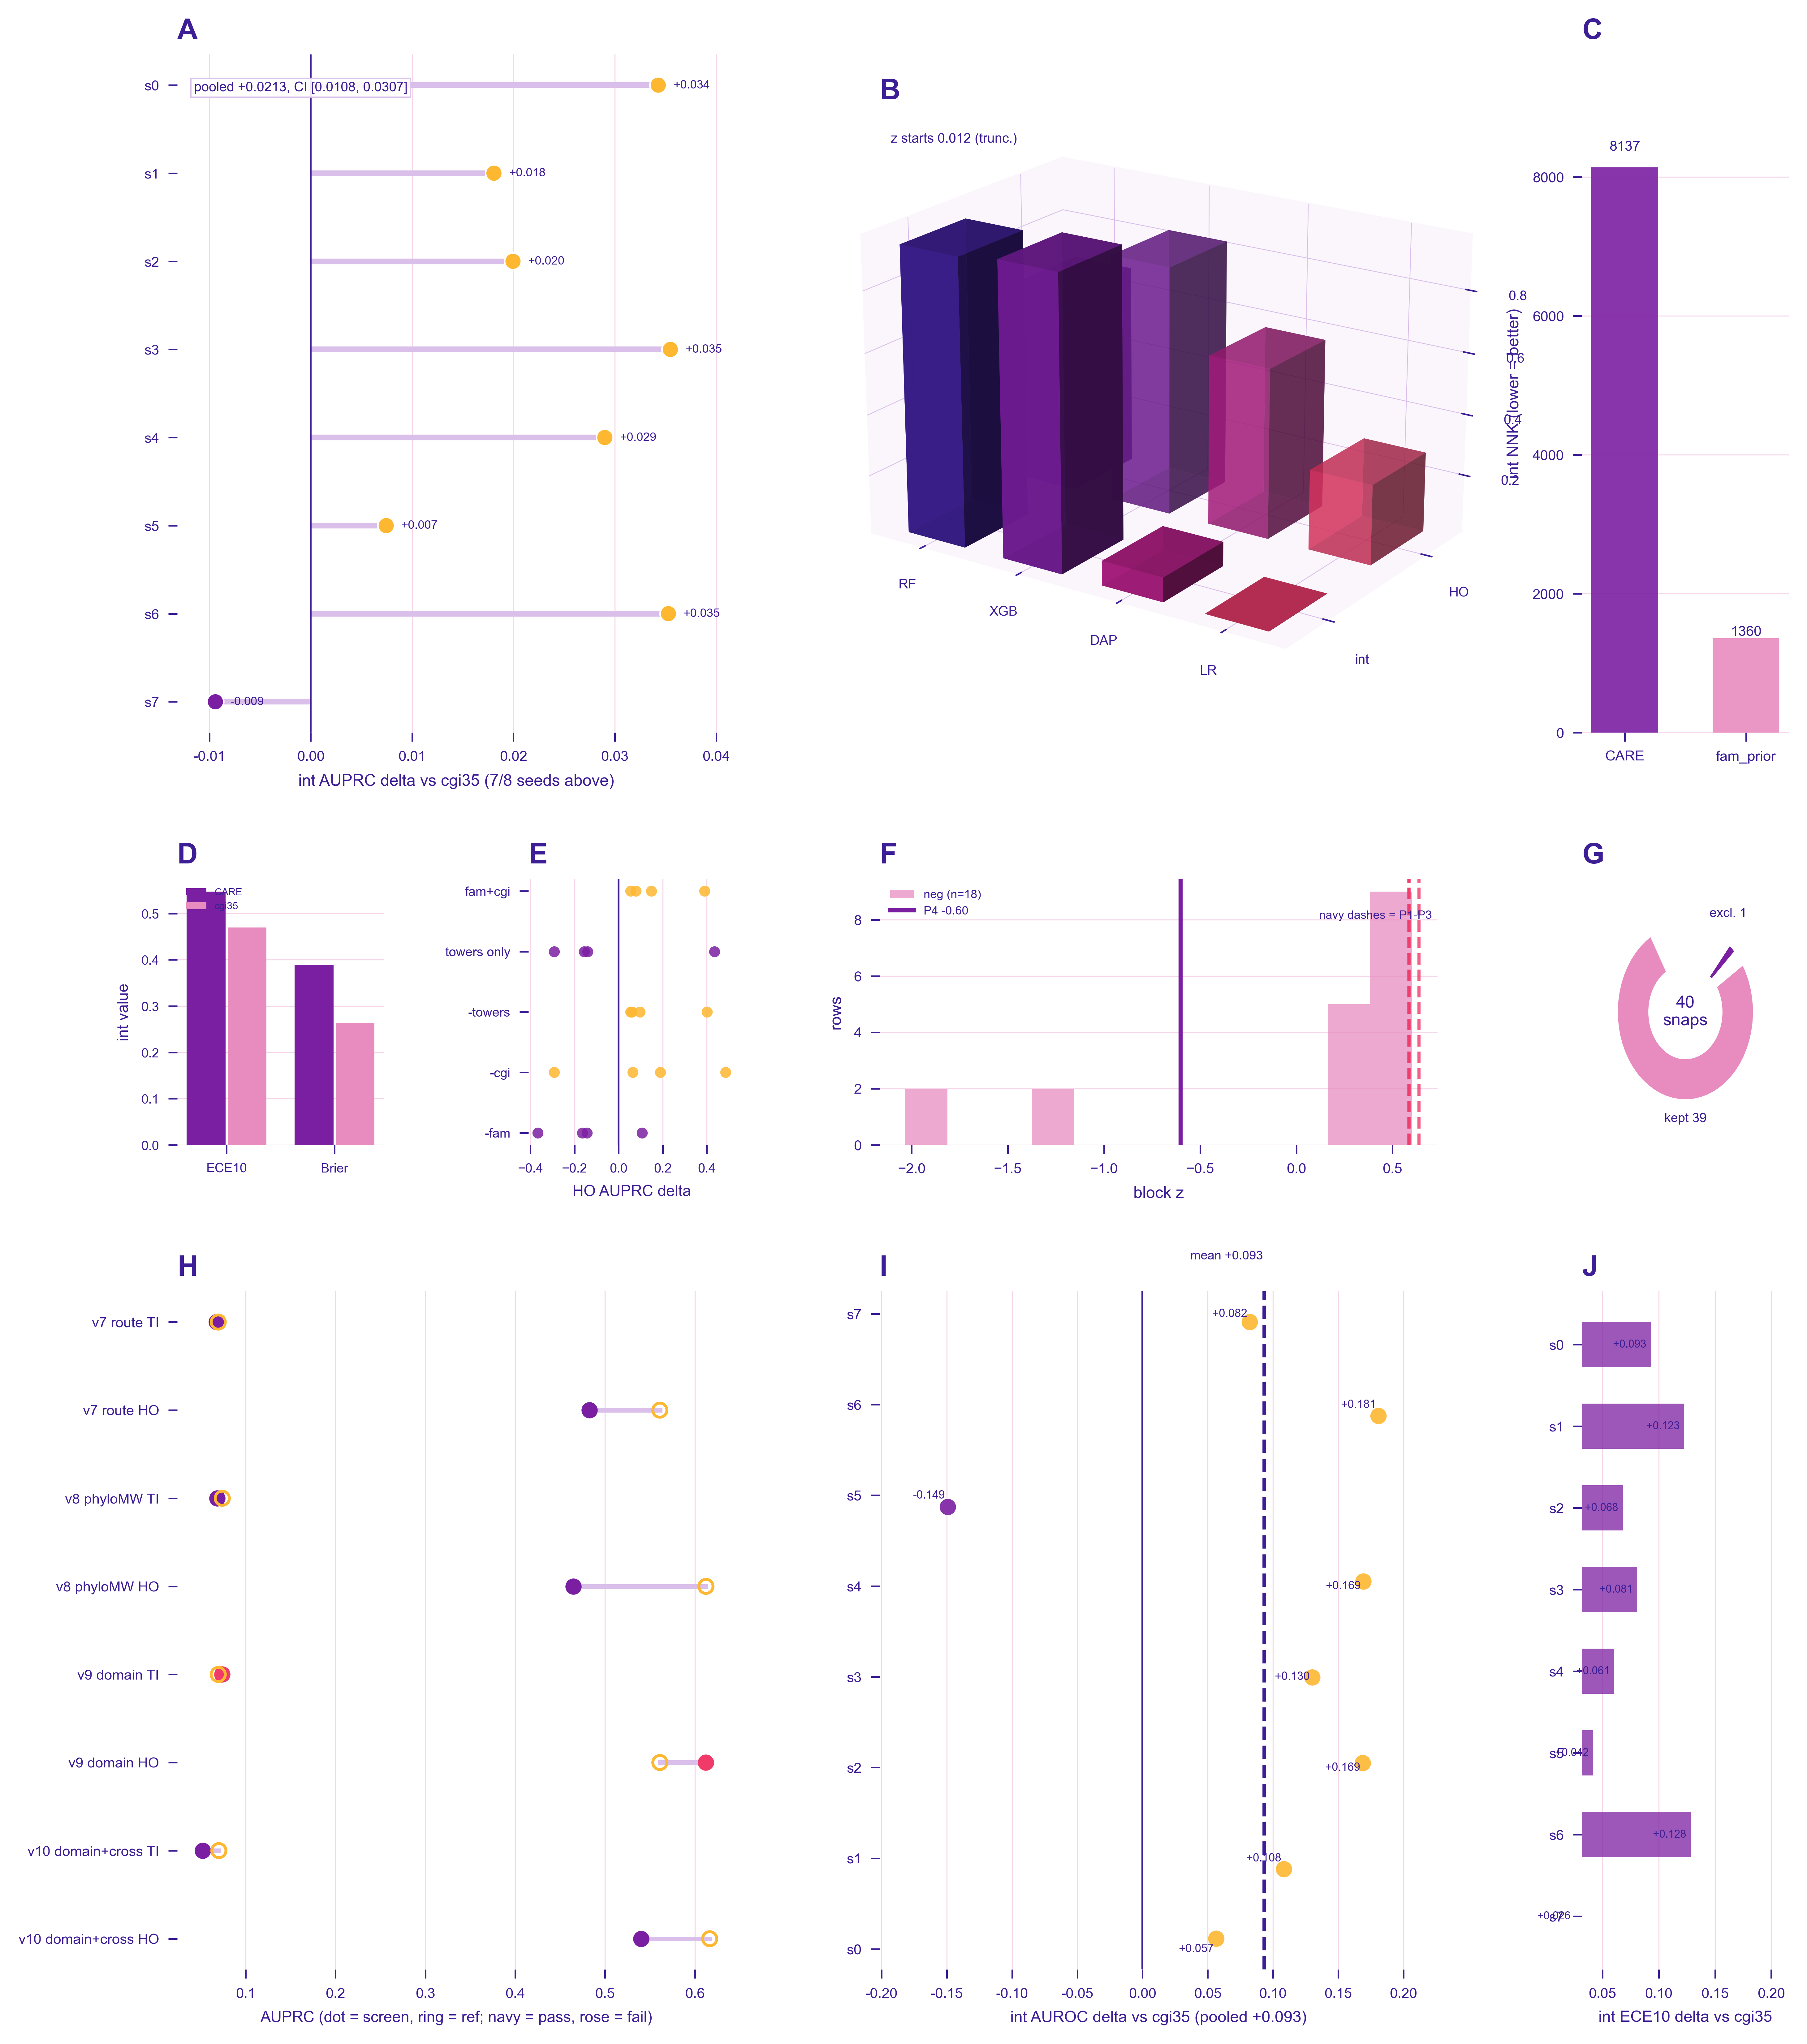
\includegraphics[width=\textwidth]{FigS1_extended.png}
\caption{\textbf{Every number the main body averages is carried here in its
per-seed form.}
(A) Internal per-seed AUPRC deltas against the screening baseline, seven of
eight seeds above with the pooled interval annotated. (B) Identity-oracle
array: four named learners across internal and holdout layers in a
truncated-z 3-D view. (C) Nearest-kin error, two bars with the lower-is-better
orientation. (D) The two carried calibration cells, ECE10 and Brier,
for model and baseline. (E) Per-seed knockout strips for five component
configurations. (F) The case-block block-$z$ distribution: three pairs recovered and the fourth
marked against them, the coverage reading that routes it to homology review. (G) The snapshot pool ring: thirty-
nine of forty carried forward. (H) All recorded screens as dumbbells
against their reference values. (I) Per-seed internal AUROC deltas with the
mean line. (J) Per-seed ECE10 deltas, the calibration cells the main body
quotes.}
\label{figS1}
\end{figure}

%% =====================================================================
\section*{S2. Protocol, corpus, and provenance}
\label{secS2}

\begin{figure}[H]
\centering
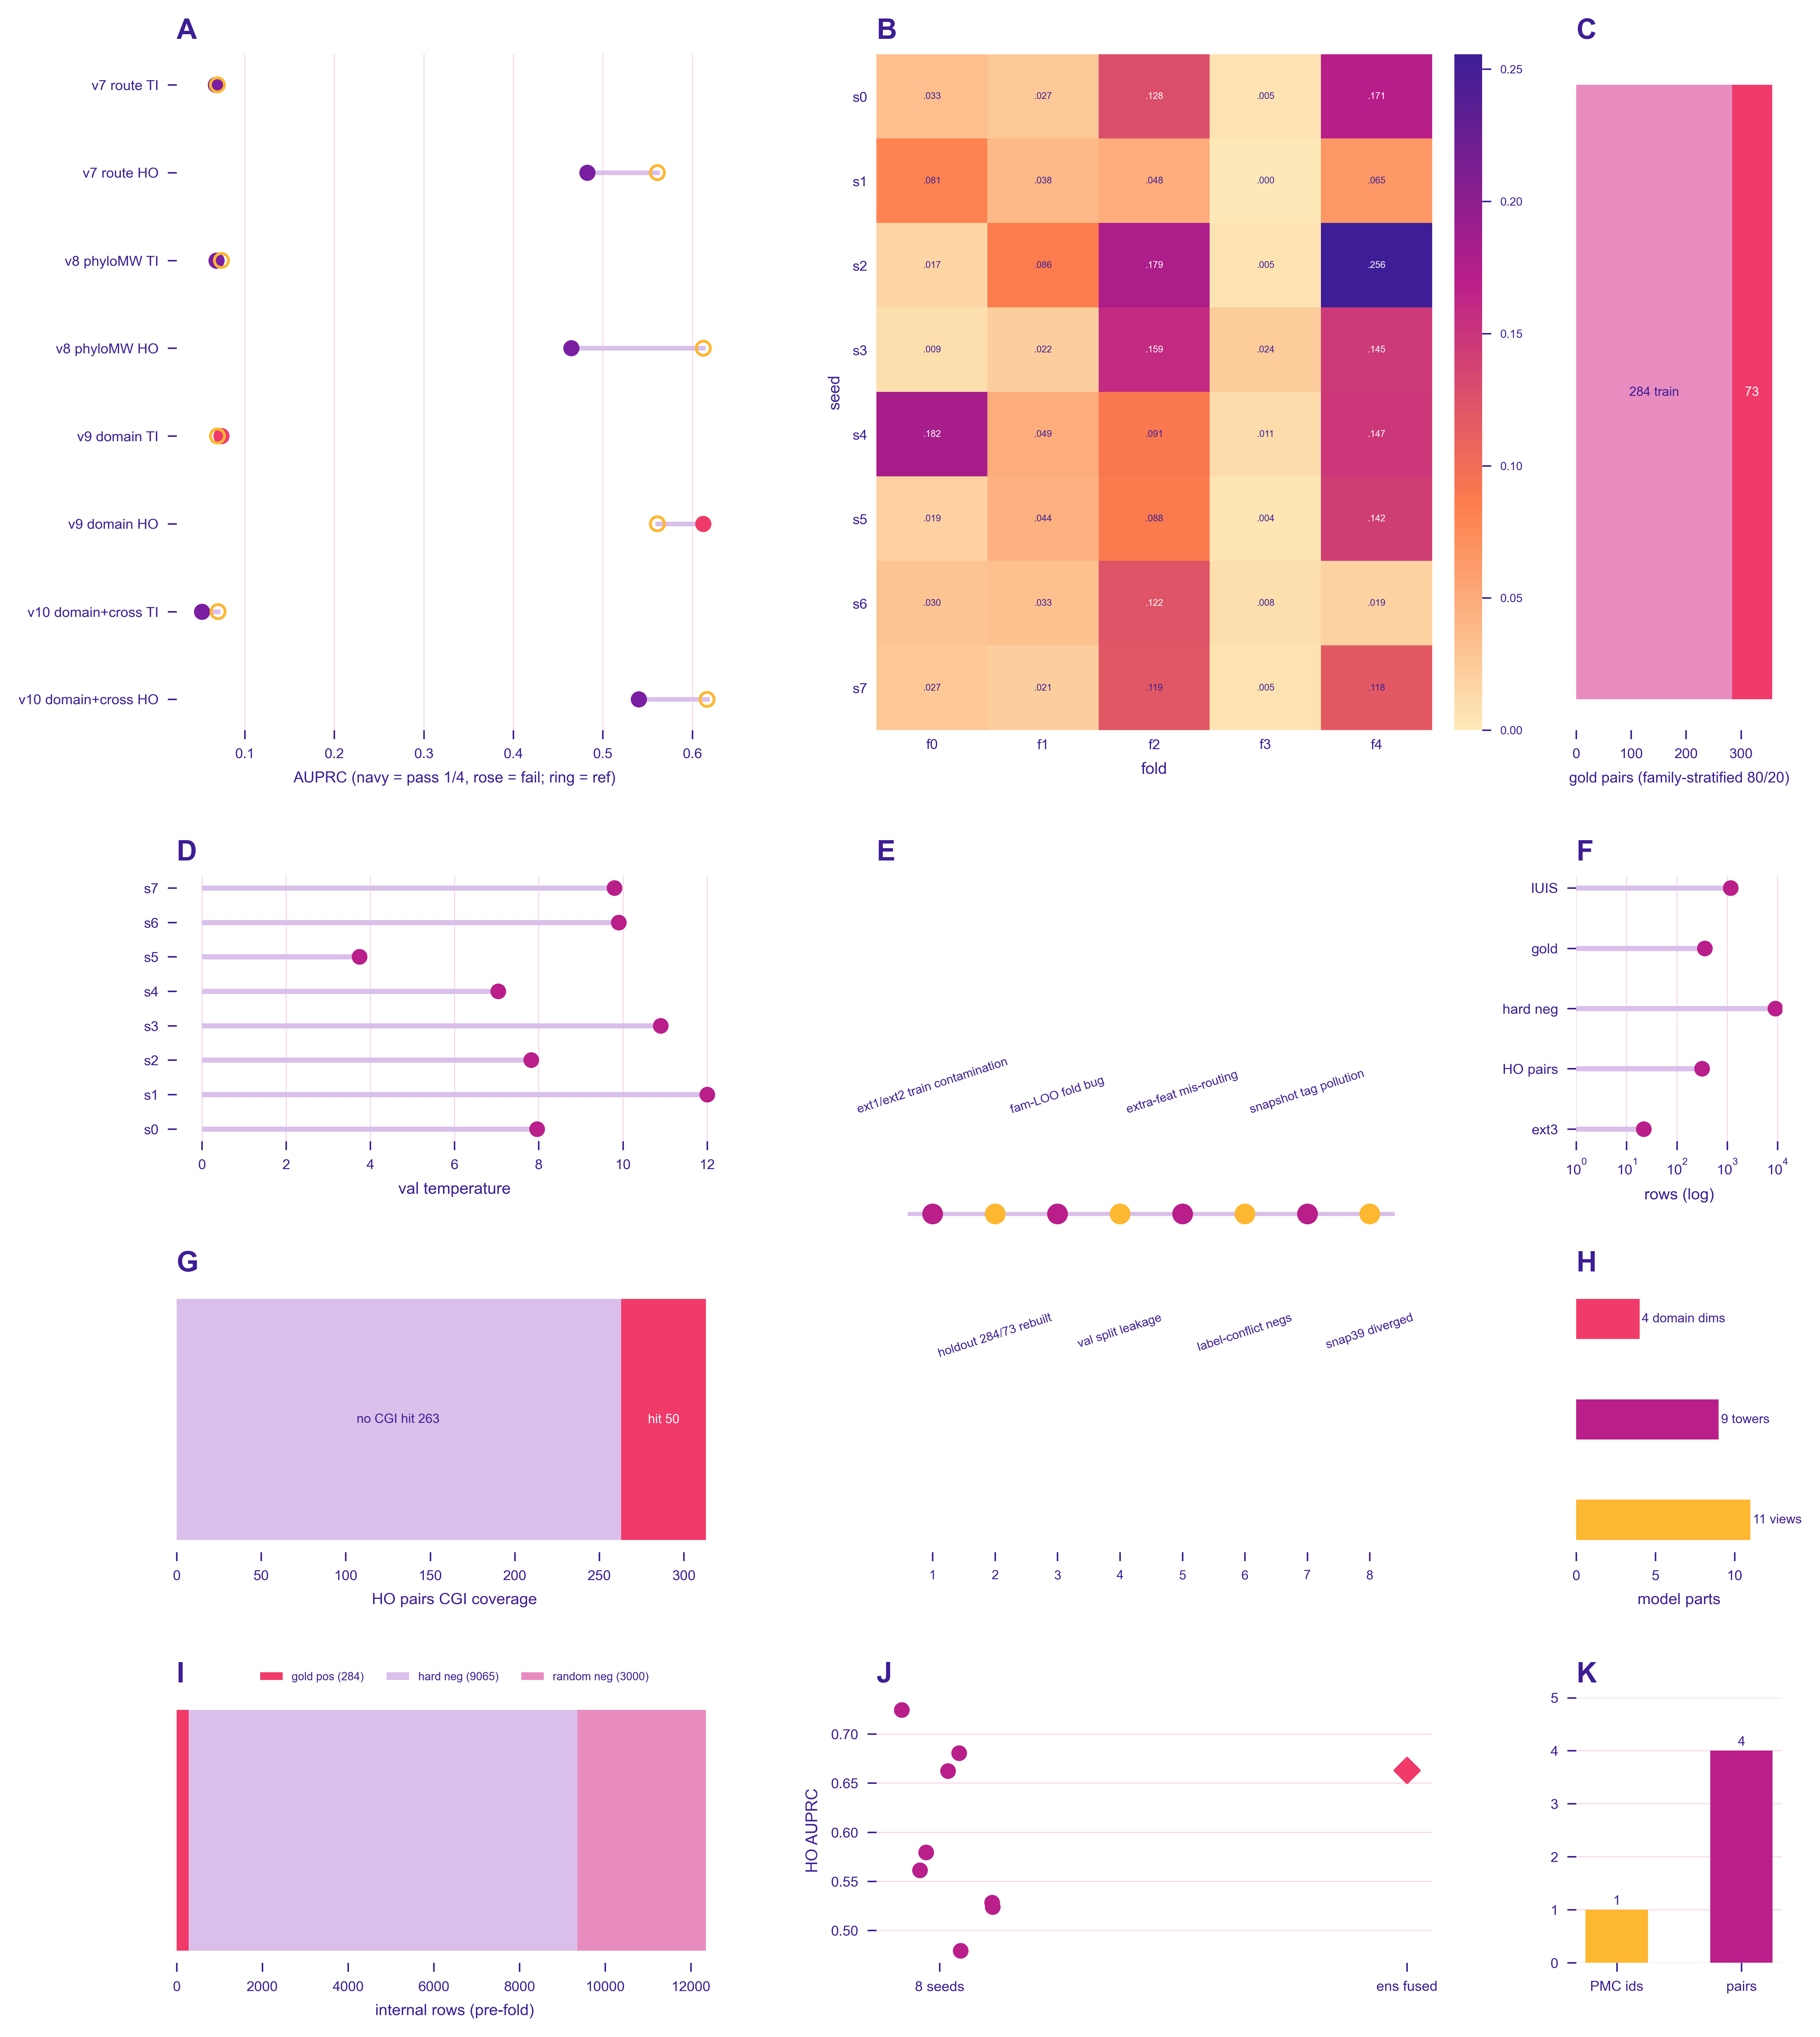
\includegraphics[width=\textwidth]{FigS2_protocol.png}
\caption{\textbf{The protocol lock is a record, and every screen on it carries a verdict.}
(A) Every recorded screen with its verdict against the reference value.
(B) The seed-by-fold internal AUPRC matrix that the fold-0 protocol consumes.
(C) The family-stratified split: 284 training gold pairs and the 73-pair
never-trained holdout. (D) The per-seed validation temperature. (E) The
protocol-fix timeline: eight items raised and cleared before the lock, in
order. (F) The data funnel from the curated resource snapshot to the scored
corpus. (G) Holdout coverage by the screening baseline: 50 pairs
reached, 263 left uncovered. (H) The model inventory: eleven views, nine towers,
four domain coordinates. (I) Class balance before the fold: 284 gold,
9{,}065 hard negatives, 3{,}000 anchors. (J) Holdout AUPRC, eight seeds
versus the fused ensemble. (K) The case-corpus provenance: source
documents against the scored pairs.}
\label{figS2}
\end{figure}

%% =====================================================================
\section*{S3. Corpus quality checks and provenance}
\label{secS3}

Three standing checks underwrite the corpus. The holdout file is stratified by
allergen family and contacted exactly once per seed after the protocol lock;
no holdout statistic participates in model, hyperparameter, or snapshot
selection. The mining pipeline flags one matched-segment record that runs past
its protein's length and routes it around the plotting stage; no reported
number draws on it, and the routing is recorded here so the corpus stays
auditable line by line. The calibration cells quoted in the main text are the
two carried cells of Figure~\ref{figS1}D, and the screen ledger of
Figure~\ref{figS2}A carries each verdict so that the component selection is
auditable row by row. Figures S1--S2 are reproduced from the frozen scoring
tables and the analysis code released with the manuscript.

%% =====================================================================
%% Manuscript declarations, carried in full so this file is self-contained.
%% These are the MDPI class back-matter commands, identical to main.tex.
%% =====================================================================
\vspace{12pt}
\authorcontributions{Conceptualization, T.S., Y.Q., P.L. and S.S.;
Methodology, T.S., J.L., Z.P. and P.L.; Software, J.L., Z.P., X.L., G.W.,
J.Z., F.Y., Z.X., Y.L., W.S., S.M., Y.C. and H.W.; Validation, J.L., Z.P.,
X.L., G.W. and J.Z.; Formal Analysis, T.S., J.L., Z.P. and P.L.;
Investigation, X.L., G.W., J.Z., F.Y., Z.X., Y.L., W.S., S.M., Y.C. and
H.W.; Resources, P.L., S.S., Y.Q. and T.S.; Data Curation, F.Y., Z.X., Y.L.,
W.S., S.M., Y.C. and H.W.; Writing--Original Draft Preparation, T.S., J.L.
and P.L.; Writing--Review \& Editing, T.S., Z.P., P.L., Y.Q. and S.S.;
Visualization, Z.P., G.W. and J.Z.; Supervision, Y.Q. and S.S.;
Project Administration, Y.Q. and S.S.; Funding Acquisition, Y.Q., P.L. and
S.S. T.S., J.L., Z.P. and P.L. contributed equally to this work and are joint
first authors. All authors have read and agreed to the published version of
the manuscript.}

\funding{This research was funded by the Shenzhen Municipal Development and
Reform Commission (Project No.: XMHT20230108023).}

\institutionalreview{Not applicable.}

\informedconsent{Not applicable.}

\dataavailability{No new experimental data were generated in this study;
the work is a computational analysis of publicly available allergen
resources. The intermediate and derived data supporting the reported
results, a real stratified data slice sufficient to reproduce the holdout
evaluation, the supplementary figures and tables, and a step-by-step usage
guide are openly available at
\url{https://github.com/SHENTongfei/DeepCARE}. All analysis and figure code,
the trained-code release, and the frozen scoring tables are available in the
same repository, whose README reproduces training, evaluation, and every
figure from the released slice with one command. The complete clinical label
set follows the distribution terms of the source databases (AllergenOnline,
the WHO/IUIS nomenclature, and the curated resources cited in Materials and
Methods) and is available from those resources. No restrictions apply to the
released slice.}

\acknowledgments{This work used publicly available data only. The clinical
cross-reaction pairs and allergen resources are openly accessible online
(AllergenOnline, the WHO/IUIS nomenclature committee, and the curated
resources cited in the main text); the authors thank the curators of these
resources.

DeepSeek was used solely for language polishing of the manuscript text
(grammar, wording and readability). No other generative AI tools were used,
and no AI tool was used for study design, data collection or analysis, code
generation, figure or table creation, interpretation of results, or writing
of the scientific content. The authors take full responsibility for the
content of this publication.}

\conflictsofinterest{The authors declare no conflicts of interest.}

\supplementary{The following supporting information can be downloaded at:
\url{www.mdpi.com/xxx/s1}. Figure S1: Extended comparisons and the full
per-metric record (10 panels); Figure S2: Protocol, corpus, and provenance
(11 panels); Section S3: Corpus quality checks and provenance. The LaTeX
source, the supplementary figures, the released data slice, and the analysis
code are also openly available at
\url{https://github.com/SHENTongfei/DeepCARE}.}

\end{document}
